\documentclass{beamer}

\usepackage[T1]{fontenc}
\usepackage[utf8]{inputenc}
\usepackage{amsmath,amssymb}
\usepackage{mathpartir}
\usepackage{stmaryrd}
\usepackage{tikz}
\usepackage{hyperref}

\definecolor{plrgprimary}{HTML}{1F2A44}
\definecolor{plrgaccent}{HTML}{3730A3}
\definecolor{plrgfunctional}{HTML}{0F766E}
\definecolor{plrgbackground}{HTML}{F8FAFC}
\definecolor{plrgtext}{HTML}{111827}

\usefonttheme{professionalfonts}

\setbeamercolor{background canvas}{bg=plrgbackground}
\setbeamercolor{title}{fg=plrgprimary}
\setbeamercolor{frametitle}{fg=plrgprimary}
\setbeamercolor{subtitle}{fg=plrgprimary}
\setbeamercolor{structure}{fg=plrgaccent}
\setbeamercolor{normal text}{fg=plrgtext}

\setbeamerfont{title}{series=\bfseries}
\setbeamerfont{frametitle}{series=\bfseries}

\setbeamertemplate{navigation symbols}{}
\setbeamertemplate{footline}[frame number]

\hypersetup{
  colorlinks=true,
  urlcolor=plrgfunctional,
}

\newcommand{\State}{\mathit{State}}
\newcommand{\Store}{\mathit{Store}}
\newcommand{\Heap}{\mathit{Heap}}
\newcommand{\Var}{\mathit{Var}}
\newcommand{\Val}{\mathit{Val}}
\newcommand{\Addr}{\mathit{Addr}}
\newcommand{\true}{\mathsf{true}}
\newcommand{\false}{\mathsf{false}}
\newcommand{\pending}{\mathsf{pending}}
\newcommand{\shot}{\mathsf{shot}}
\newcommand{\invalid}{\mathord{\lightning}}

\title{Program Logic}
\subtitle{Introduction to Program Verification --- Part 2}
\author{Jaemin Hong}
\date{}

\begin{document}

\begin{frame}
  \titlepage
\end{frame}

\begin{frame}{Program Verification}
  \begin{itemize}
    \item How can we state properties of programs?
    \item Can we have proof techniques that can be applied to a wide range of programs?
  \end{itemize}
\end{frame}

\begin{frame}{Today's Topics}
  \begin{itemize}
    \item Preconditions and postconditions
    \item Program logic
      \begin{itemize}
        \item Hoare logic
        \item Separation logic
          \begin{itemize}
            \item Separating conjunction
            \item Frame rule
          \end{itemize}
        \item Iris
          \begin{itemize}
            \item Resource algebras
            \item Invariants
          \end{itemize}
      \end{itemize}
  \end{itemize}
\end{frame}

\begin{frame}{Inference Rules}
  \[
    \inferrule{premise_1 \quad premise_2 \quad \cdots}
              {conclusion}
  \]
  means ``if all premises can be proven, then the conclusion can be proven.''
\end{frame}

\begin{frame}{Inference Rules: Example}
  \begin{itemize}
    \item Modus ponens
  \end{itemize}
  \[
    \inferrule{A \\ A \Rightarrow B}{B}
  \]
\end{frame}

\begin{frame}{Imp Language: Syntax}
  \[
  \begin{aligned}
    a &\mathrel{::=} n \mathbin{|} x
      \mathbin{|} a\mathbin{\texttt{+}}a
      \mathbin{|} a\mathbin{\texttt{-}}a
      \mathbin{|} a\mathbin{\texttt{*}}a
      \mathbin{|} \texttt{...} \\
    b &\mathrel{::=} \texttt{true}
      \mathbin{|} \texttt{false}
      \mathbin{|} a\mathbin{\texttt{==}}a
      \mathbin{|} a\mathbin{\texttt{<=}}a
      \mathbin{|} b\mathbin{\texttt{\&\&}}b
      \mathbin{|} \texttt{...} \\
    c &\mathrel{::=} \texttt{skip}
      \mathbin{|} x\mathbin{\texttt{:=}}a
      \mathbin{|} c\mathbin{\texttt{;}}c
      \mathbin{|} \texttt{if }b\texttt{ then }c\texttt{ else }c
      \mathbin{|} \texttt{while }b\texttt{ do }c
  \end{aligned}
  \]
\end{frame}

\begin{frame}{Imp Language: Semantics (Arithmetic)}
  \[
    \State = \Var \to \mathbb{Z}
  \]

  \begin{mathpar}
    \inferrule{ }{S \vdash n \Rightarrow n}

    \inferrule{ }{S \vdash x \Rightarrow S(x)}

    \inferrule{S \vdash a_{1} \Rightarrow n_{1} \\
               S \vdash a_{2} \Rightarrow n_{2}}
              {S \vdash a_{1}\mathbin{\texttt{+}}a_{2}
                 \Rightarrow n_{1}+n_{2}}
  \end{mathpar}
\end{frame}

\begin{frame}{Imp Language: Semantics (Boolean)}
  \begin{mathpar}
    \inferrule{ }{S \vdash \texttt{true} \Rightarrow \true}

    \inferrule{S \vdash a_{1} \Rightarrow n_{1} \\
               S \vdash a_{2} \Rightarrow n_{2}}
              {S \vdash a_{1}\mathbin{\texttt{==}}a_{2}
                 \Rightarrow n_{1}=n_{2}}

    \inferrule{S \vdash b_{1} \Rightarrow B_{1} \\
               S \vdash b_{2} \Rightarrow B_{2}}
              {S \vdash b_{1}\mathbin{\texttt{\&\&}}b_{2}
                 \Rightarrow B_{1}\land B_{2}}
  \end{mathpar}
\end{frame}

\begin{frame}{Imp Language: Semantics (Command)}
  \begin{mathpar}
    \inferrule{ }{S \vdash \texttt{skip} \Rightarrow S}

    \inferrule{S \vdash a \Rightarrow n}
              {S \vdash x\mathbin{\texttt{:=}}a \Rightarrow S[x\mapsto n]}

    \inferrule{S_{0} \vdash c_{1} \Rightarrow S_{1} \\
               S_{1} \vdash c_{2} \Rightarrow S_{2}}
              {S_{0} \vdash c_{1}\mathbin{\texttt{;}}c_{2} \Rightarrow S_{2}}
  \end{mathpar}
\end{frame}

\begin{frame}{Imp Language: Semantics (Command)}
  \begin{mathpar}
    \inferrule{S_{0} \vdash b \Rightarrow \texttt{true} \\
               S_{0} \vdash c_{1} \Rightarrow S_{1}}
              {S_{0} \vdash \texttt{if }b\texttt{ then }c_{1}
                 \texttt{ else }c_{2} \Rightarrow S_{1}}

    \inferrule{S_{0} \vdash b \Rightarrow \texttt{false} \\
               S_{0} \vdash c_{2} \Rightarrow S_{2}}
              {S_{0} \vdash \texttt{if }b\texttt{ then }c_{1}
                 \texttt{ else }c_{2} \Rightarrow S_{2}}

    \inferrule{S_{0} \vdash b \Rightarrow \texttt{true} \\
               S_{0} \vdash c \Rightarrow S_{1} \\
               S_{1} \vdash \texttt{while }b\texttt{ do }c \Rightarrow S_{2}}
              {S_{0} \vdash \texttt{while }b\texttt{ do }c \Rightarrow S_{2}}

    \inferrule{S \vdash b \Rightarrow \texttt{false}}
              {S \vdash \texttt{while }b\texttt{ do }c \Rightarrow S}
  \end{mathpar}
\end{frame}

\begin{frame}{Assertions}
  \begin{itemize}
    \item An \emph{assertion} is a logical claim about the state of a program's memory.
    \item Formally, an assertion is a predicate over $\State$.
  \end{itemize}
\end{frame}

\begin{frame}{Assertions: Examples}
  \begin{itemize}
    \item $S \mapsto \mathsf{True}$, or $\mathsf{True}$ if it is clear that this expresses an assertion.
    \item $S \mapsto \mathsf{False}$, or $\mathsf{False}$.
    \item $S \mapsto S(\texttt{x})=5$, or $\texttt{x}=5$.
    \item $S \mapsto S(\texttt{x})=5 \land S(\texttt{y})=7$, or
      $\texttt{x}=5 \land \texttt{y}=7$.
  \end{itemize}
\end{frame}

\begin{frame}{Assertion Implication}
  \begin{itemize}
    \item Where $P$ and $Q$ are assertions, $P$ \emph{implies} $Q$ iff, whenever
      $P$ holds in some state, $Q$ also holds.
    \item $P \Rightarrow Q$ iff $\forall S.\ P(S) \to Q(S)$.
    \item Examples:
      \begin{itemize}
        \item $\texttt{x}=5 \land \texttt{y}=7$ implies $\texttt{x}=5$.
        \item Any assertion implies $\mathsf{True}$.
        \item $\mathsf{False}$ implies any assertion.
      \end{itemize}
  \end{itemize}
\end{frame}

\begin{frame}{Hoare Triples}
  \begin{itemize}
    \item A \emph{Hoare triple} is a claim about the state before and after executing a command.
    \item A standard notation is $\{P\}\ c\ \{Q\}$, meaning
      \begin{itemize}
        \item If $c$ begins execution in a state satisfying $P$ (precondition)
        \item and if $c$ terminates,
        \item then the final state satisfies $Q$ (postcondition).
      \end{itemize}
  \end{itemize}
\end{frame}

\begin{frame}{Hoare Triples: Examples}
  \begin{itemize}
    \item $\{\mathsf{True}\}\ \texttt{x := 5}\ \{\texttt{x}=5\}$ is valid.
    \item $\{\texttt{x}=5\}\ \texttt{y := 10}\ \{\texttt{x}=5\}$ is valid.
    \item $\{\mathsf{False}\}\ \texttt{x := 5}\ \{\texttt{x}=10\}$ is valid.
    \item $\{\mathsf{True}\}\ \texttt{x := 5}\ \{\mathsf{False}\}$ is not valid.
    \item $\{\texttt{x}=5\}\ \texttt{x := 7}\ \{\texttt{x}=5\}$ is not valid.
  \end{itemize}
\end{frame}

\begin{frame}{Program Verification with Hoare Triples}
  \begin{itemize}
    \item A \emph{specification} of a program $prog$ can be stated with a
      precondition $P$ and a postcondition $Q$.
    \item Verifying $prog$ with respect to the specification means proving that
      the Hoare triple $\{P\}\ prog\ \{Q\}$ is valid.
  \end{itemize}
\end{frame}

\begin{frame}{Hoare Logic}
  \begin{itemize}
    \item Hoare logic provides a compositional method for proving the validity of Hoare triples.
    \item The structure of a program's correctness proof mirrors the structure of the program.
    \item Proposed by Tony Hoare in 1969\footnote{An axiomatic basis for computer programming (Hoare, 1969)} and subsequently refined by others.
  \end{itemize}
\end{frame}

\begin{frame}{Hoare Logic: Skip}
  \[
    \inferrule{ }{\{P\}\ \texttt{skip}\ \{P\}}
  \]
\end{frame}

\begin{frame}{Hoare Logic: Sequencing}
  \[
    \inferrule{\{P\}\ c_{1}\ \{Q\} \\
               \{Q\}\ c_{2}\ \{R\}}
              {\{P\}\ c_{1}\mathbin{\texttt{;}}c_{2}\ \{R\}}
  \]
\end{frame}

\begin{frame}{Hoare Logic: Assignments}
  \[
    \inferrule{ }{\{P[x\mapsto a]\}\ x\mathbin{\texttt{:=}}a\ \{P\}}
  \]
  \begin{itemize}
    \item Intuition: If we want $x\mathbin{\texttt{:=}}a$ to terminate in a
      state that satisfies $P$, then it suffices to start in a state that also
      satisfies $P$, except where every occurrence of $x$ is substituted with $a$.
  \end{itemize}
\end{frame}

\begin{frame}{Hoare Logic: Assignments --- Examples}
  \begin{itemize}
    \item $\{3=3\}\ \texttt{x := 3}\ \{\texttt{x}=3\}$
    \item $\{\texttt{x}+1<5\}\ \texttt{x := x + 1}\ \{\texttt{x}<5\}$
    \item $\{\texttt{y}=1\}\ \texttt{x := y}\ \{\texttt{x}=1\}$
  \end{itemize}
\end{frame}

\begin{frame}{Hoare Logic: Consequence}
  \[
    \inferrule{P \Rightarrow P' \\
               \{P'\}\ c\ \{Q'\} \\
               Q' \Rightarrow Q}
              {\{P\}\ c\ \{Q\}}
  \]
\end{frame}

\begin{frame}{Hoare Logic: Consequence --- Example}
  \[
    \inferrule{\mathsf{True}\Rightarrow 3=3 \\
               \{3=3\}\ \texttt{x := 3}\ \{\texttt{x}=3\} \\
               \texttt{x}=3\Rightarrow\texttt{x}=3}
              {\{\mathsf{True}\}\ \texttt{x := 3}\ \{\texttt{x}=3\}}
  \]
\end{frame}

\begin{frame}{Hoare Logic: Conditionals}
  \[
    \inferrule{\{P\land b\}\ c_{1}\ \{Q\} \\
               \{P\land\lnot b\}\ c_{2}\ \{Q\}}
              {\{P\}\ \texttt{if }b\texttt{ then }c_{1}
                 \texttt{ else }c_{2}\ \{Q\}}
  \]
\end{frame}

\begin{frame}{Hoare Logic: Conditionals --- Example}
  \begin{itemize}
    \item Let $c$ be \texttt{if x == 0 then y := 2 else y := x + 1}.
  \end{itemize}

    \scriptsize
  \[
  \inferrule
    {\mathsf{True}\land\texttt{x}=0 \Rightarrow \texttt{x}=0\land2=2 \\
     \{\texttt{x}=0\land2=2\}\ \texttt{y := 2}\
       \{\texttt{x}=0\land\texttt{y}=2\} \\
     \texttt{x}=0\land\texttt{y}=2 \Rightarrow \texttt{x}\leq\texttt{y}}
    {\{\mathsf{True}\land\texttt{x}=0\}\ \texttt{y := 2}\
       \{\texttt{x}\leq\texttt{y}\}}
  \]

  \[
  \inferrule
    {\mathsf{True}\land\lnot\texttt{x}=0 \Rightarrow
       \texttt{x}+1=\texttt{x}+1 \\
     \{\texttt{x}+1=\texttt{x}+1\}\ \texttt{y := x + 1}\
       \{\texttt{y}=\texttt{x}+1\} \\
     \texttt{y}=\texttt{x}+1 \Rightarrow \texttt{x}\leq\texttt{y}}
    {\{\mathsf{True}\land\lnot\texttt{x}=0\}\ \texttt{y := x + 1}\
       \{\texttt{x}\leq\texttt{y}\}}
  \]

  \[
  \inferrule
    {\{\mathsf{True}\land\texttt{x}=0\}\ \texttt{y := 2}\
       \{\texttt{x}\leq\texttt{y}\} \\
     \{\mathsf{True}\land\lnot\texttt{x}=0\}\ \texttt{y := x + 1}\
       \{\texttt{x}\leq\texttt{y}\}}
    {\{\mathsf{True}\}\ c\ \{\texttt{x}\leq\texttt{y}\}}
  \]
\end{frame}

\begin{frame}{Hoare Logic: Conditionals --- Example}
  \small
  \[
  \begin{aligned}
    &\{\mathsf{True}\} \\
    &\texttt{if x == 0 then} \\
    &\quad \{\mathsf{True}\land\texttt{x}=0\}\Rightarrow \\
    &\quad \{\texttt{x}=0\land2=2\} \\
    &\quad \texttt{y := 2} \\
    &\quad \{\texttt{x}=0\land\texttt{y}=2\}\Rightarrow \\
    &\quad \{\texttt{x}\leq\texttt{y}\} \\
    &\texttt{else} \\
    &\quad \{\mathsf{True}\land\lnot\texttt{x}=0\}\Rightarrow \\
    &\quad \{\texttt{x}+1=\texttt{x}+1\} \\
    &\quad \texttt{y := x + 1} \\
    &\quad \{\texttt{y}=\texttt{x}+1\}\Rightarrow \\
    &\quad \{\texttt{x}\leq\texttt{y}\} \\
    &\{\texttt{x}\leq\texttt{y}\}
  \end{aligned}
  \]
\end{frame}

\begin{frame}{Hoare Logic: While Loops}
  \[
    \inferrule{\{P\land b\}\ c\ \{P\}}
              {\{P\}\ \texttt{while }b\texttt{ do }c\
                 \{P\land\lnot b\}}
  \]
  \begin{itemize}
    \item $P$ is called a \emph{loop invariant}.
  \end{itemize}
\end{frame}

\begin{frame}{Hoare Logic: While Loops --- Example}
  \[
  \begin{aligned}
    &\{\texttt{x}=0\}\Rightarrow \\
    &\{\texttt{x}\leq3\} \\
    &\texttt{while x <= 2 do} \\
    &\quad \{\texttt{x}\leq3\land\texttt{x}\leq2\}\Rightarrow \\
    &\quad \{\texttt{x}+1\leq3\} \\
    &\quad \texttt{x := x + 1} \\
    &\quad \{\texttt{x}\leq3\} \\
    &\{\texttt{x}\leq3\land\lnot\texttt{x}\leq2\}\Rightarrow \\
    &\{\texttt{x}=3\}
  \end{aligned}
  \]
\end{frame}

\begin{frame}{Hoare Logic}
  \begin{itemize}
    \item Soundness: any Hoare triple derived by the inference rules of Hoare logic is valid.
    \item Completeness: if a Hoare triple is valid, then it can be derived by the inference rules of Hoare logic.
    \item Undecidability: there is no algorithm that can determine whether an arbitrary Hoare triple is valid.
  \end{itemize}
\end{frame}

\begin{frame}{Verifying Programs that Manipulate Pointers}
  \begin{itemize}
    \item Is the following valid?
      $\{\texttt{x}\mapsto0\land\texttt{y}\mapsto0\}\
       \texttt{*x := 1}\
       \{\texttt{x}\mapsto1\land\texttt{y}\mapsto0\}$
      \begin{itemize}
        \item Here, $x\mapsto v$ means that $x$ is a pointer to a memory cell containing $v$.
      \end{itemize}
  \end{itemize}
\end{frame}

\begin{frame}{Separation Logic}
  \begin{itemize}
    \item Program logic that supports reasoning about programs that manipulate pointers.
    \item Key ideas: separating conjunction and frame rule.
    \item Proposed by Peter O'Hearn, John Reynolds, and Hongseok Yang in 2001\footnote{Local reasoning about programs that alter data structures (O'Hearn et al., 2001)}.
  \end{itemize}
\end{frame}

\begin{frame}{Memory Model}
  \begin{itemize}
    \item $\Store = \Var \to \Val$
    \item $\Heap = \displaystyle\bigcup_{A\overset{\mathsf{fin}}{\subseteq}\Addr}
      (A\to\Val)$
    \item $\State = \Store \times \Heap$
  \end{itemize}
\end{frame}

\begin{frame}{Notations for Heaps}
  \begin{itemize}
    \item $H_{1}\perp H_{2}$ means
      $\operatorname{dom}(H_{1})\cap\operatorname{dom}(H_{2})=\emptyset$.
    \item $H_{1}\uplus H_{2}$ is the union of $H_{1}$ and $H_{2}$ if
      $H_{1}\perp H_{2}$.
  \end{itemize}
\end{frame}

\begin{frame}{Assertions}
  \begin{itemize}
    \item An \emph{assertion} is a logical claim about the state of a program's memory.
    \item Formally, an assertion is a predicate over $\State$.
  \end{itemize}
\end{frame}

\begin{frame}{Assertions in Separation Logic}
  \begin{itemize}
    \item The assertion $\mathsf{emp}$ represents
      $(S,H)\mapsto\operatorname{dom}(H)=\emptyset$.
    \item A \emph{points-to} assertion $x\mapsto v$ represents
      $(S,H)\mapsto\operatorname{dom}(H)=\{S(x)\}\land H(S(x))=v$.
    \item A \emph{separating conjunction} $P*Q$ represents
      $(S,H)\mapsto\exists H_{1},H_{2}.\ H_{1}\perp H_{2}\land
      H_{1}\uplus H_{2}=H\land P(S,H_{1})\land Q(S,H_{2})$.
    \item A \emph{separating implication} (\emph{magic wand}) $P\mathbin{-\!*}Q$
      represents $(S,H)\mapsto\forall H'.\ H'\perp H\land P(S,H')
      \to Q(S,H\uplus H')$.
  \end{itemize}
\end{frame}

\begin{frame}{Separating Conjunction: Examples}
  \centering
  \resizebox{.94\textwidth}{!}{%
  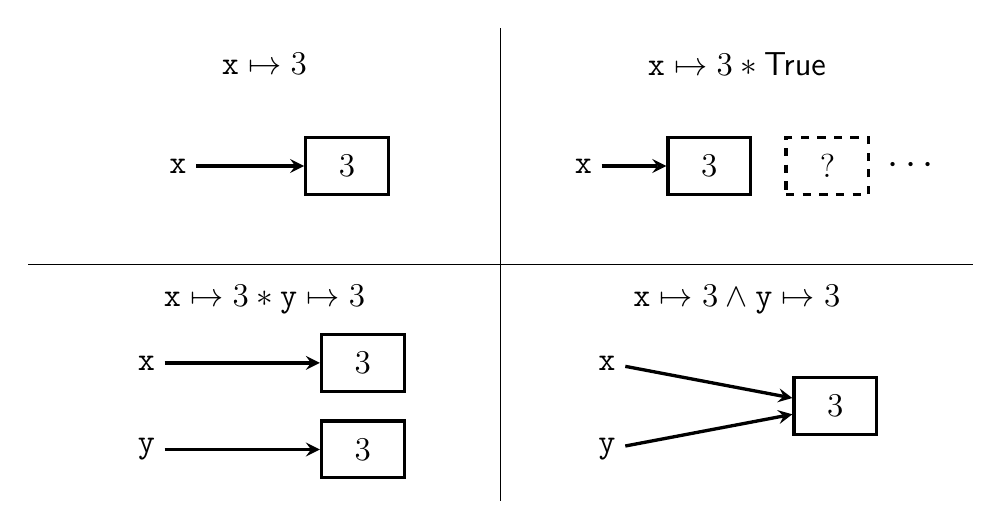
\begin{tikzpicture}[
    >=stealth,
    var/.style={font=\ttfamily\large},
    cell/.style={draw=black, very thick,
      minimum width=1.05cm, minimum height=.72cm, font=\large},
    ptr/.style={->, very thick, draw=black},
    formula/.style={font=\large},
  ]
    \draw[thin] (6,0) -- (6,6);
    \draw[thin] (0,3) -- (12,3);

    \node[formula] at (3,5.55) {$\texttt{x}\mapsto3$};
    \node[var] (x1) at (1.9,4.25) {x};
    \node[cell] (x1cell) at (4.05,4.25) {$3$};
    \draw[ptr] (x1) -- (x1cell);

    \node[formula] at (9,5.55) {$\texttt{x}\mapsto3*\mathsf{True}$};
    \node[var] (x2) at (7.05,4.25) {x};
    \node[cell] (x2cell) at (8.65,4.25) {$3$};
    \draw[ptr] (x2) -- (x2cell);
    \node[cell,dashed] at (10.15,4.25) {$?$};
    \node[font=\Large] at (11.25,4.25) {$\cdots$};

    \node[formula] at (3,2.55)
      {$\texttt{x}\mapsto3*\texttt{y}\mapsto3$};
    \node[var] (x3) at (1.5,1.75) {x};
    \node[var] (y3) at (1.5,.65) {y};
    \node[cell] (x3cell) at (4.25,1.75) {$3$};
    \node[cell] (y3cell) at (4.25,.65) {$3$};
    \draw[ptr] (x3) -- (x3cell);
    \draw[ptr] (y3) -- (y3cell);

    \node[formula] at (9,2.55)
      {$\texttt{x}\mapsto3\land\texttt{y}\mapsto3$};
    \node[var] (x4) at (7.35,1.75) {x};
    \node[var] (y4) at (7.35,.65) {y};
    \node[cell] (xycell) at (10.25,1.2) {$3$};
    \draw[ptr] (x4) -- (xycell);
    \draw[ptr] (y4) -- (xycell);
  \end{tikzpicture}
  }
\end{frame}

\begin{frame}{Separating Conjunction: Examples}
  \begin{itemize}
    \item $\texttt{x}\mapsto3*\texttt{x}\mapsto3$
      \begin{itemize}
        \item Equivalent to $\mathsf{False}$
      \end{itemize}
    \item $\texttt{x}\mapsto3\land\texttt{y}\mapsto5$
      \begin{itemize}
        \item Equivalent to $\mathsf{False}$
      \end{itemize}
  \end{itemize}
\end{frame}

\begin{frame}{Separation Logic is Substructural}
  \begin{itemize}
    \item In general, $P$ does not imply $P*P$.
  \end{itemize}
\end{frame}

\begin{frame}{Pure Assertions}
  \begin{itemize}
    \item An assertion is \emph{pure} if it is independent of the heap.
      \begin{itemize}
        \item Syntactically, an assertion is pure if it does not contain
          $\mathsf{emp}$ or $\mapsto$.
      \end{itemize}
    \item When assertions are pure, separating conjunction behaves like ordinary conjunction.
      \begin{itemize}
        \item $P\land Q$ implies $P*Q$ if $P$ or $Q$ is pure.
        \item $P*Q$ implies $P\land Q$ if $P$ and $Q$ are pure.
      \end{itemize}
  \end{itemize}
\end{frame}

\begin{frame}{Separation Logic: Frame Rule}
  \[
    \inferrule{\{P\}\ c\ \{Q\}}
              {\{P*R\}\ c\ \{Q*R\}}
  \]
  where no variable in $R$ is modified by $c$.

  \begin{itemize}
    \item The key to \emph{local reasoning} about the heap.
  \end{itemize}
\end{frame}

\begin{frame}{Separation Logic: Allocation}
  \[
    \inferrule{ }{\{\mathsf{emp}\}\
      x\mathbin{\texttt{:=}}\texttt{alloc(}e\texttt{)}\ \{x\mapsto e\}}
  \]
\end{frame}

\begin{frame}{Separation Logic: Mutation}
  \[
    \inferrule{ }{\{x\mapsto v\}\
      \texttt{*}x\mathbin{\texttt{:=}}e\ \{x\mapsto e\}}
  \]
\end{frame}

\begin{frame}{Separation Logic: Deallocation}
  \[
    \inferrule{ }{\{x\mapsto v\}\
      \texttt{free(}x\texttt{)}\ \{\mathsf{emp}\}}
  \]
\end{frame}

\begin{frame}{Concurrent Separation Logic (CSL)\footnote{Resources, concurrency, and local reasoning (O'Hearn, 2007)}}
  \[
    \inferrule{\{P\}\ c_{1}\ \{Q\} \\
               \{R\}\ c_{2}\ \{S\}}
              {\{P*R\}\ c_{1}\mathbin{\texttt{||}}c_{2}\ \{Q*S\}}
  \]
  where neither command modifies a variable occurring in the other command or
  its specification.
\end{frame}

\begin{frame}{Extending CSL}
  \begin{quote}
    In recent years, separation logic has brought great advances in the world of
    verification. However, there is a disturbing trend for each new library or
    concurrency primitive to require a new separation logic.\footnote{The next
    700 separation logics (Parkinson, 2010)}
  \end{quote}
\end{frame}

\begin{frame}{Iris\footnote{Iris: Monoids and invariants as
      an orthogonal basis for concurrent reasoning (Jung et al., 2015)}}
  \begin{itemize}
    \item Iris is a higher-order concurrent separation logic with user-defined
      resource algebras and invariants.
  \end{itemize}
\end{frame}

\begin{frame}{Iris: Example}
  \small
  \begin{itemize}
    \item Code:
  \end{itemize}
  \[
  \begin{aligned}
    \texttt{mk\_oneshot} \triangleq{}& \lambda\,\texttt{\_. let x = alloc(inl(0)) in} \\
      &\{\ \texttt{tryset = }\lambda\,\texttt{n. CAS(x, inl(0), inr(n)),} \\
      &\phantom{\{}\ \texttt{check = }\lambda\,\texttt{\_. let y = *x in }\lambda\,\texttt{\_.} \\
      &\phantom{\{\ \texttt{check = }}\texttt{match y, *x with} \\
      &\phantom{\{\ \texttt{check = }}\texttt{| inl(\_), \_ => ()} \\
      &\phantom{\{\ \texttt{check = }}\texttt{| inr(\_), inl(\_) => assert(false)} \\
      &\phantom{\{\ \texttt{check = }}\texttt{| inr(n), inr(m) => assert(n = m)} \\
      &\phantom{\{\ \texttt{check = }}\texttt{end}
  \end{aligned}
  \]
  \begin{itemize}
    \item Specification:
  \end{itemize}
  \[
  \begin{aligned}
    \{\mathsf{True}\}\ \texttt{mk\_oneshot()}\
    \{\texttt{c}.\ \forall\texttt{v}.\;&
      \{\mathsf{True}\}\ \texttt{c.tryset(v)}\
        \{\texttt{w}.\ \texttt{w}\in\{\true,\false\}\}\ \ast \\
      &\{\mathsf{True}\}\ \texttt{c.check()}\
        \{\texttt{f}.\ \{\mathsf{True}\}\ \texttt{f ()}\ \{\mathsf{True}\}\}\ \}
  \end{aligned}
  \]
  \footnotetext{Iris from the ground up: A modular foundation for higher-order
  concurrent separation logic (Jung et al., 2018)}
\end{frame}

\begin{frame}{Iris: Example --- Resource Algebra (Elements)}
  \begin{itemize}
    \item We can define a resource algebra $M$ to reflect the state of the
      physical location $\texttt{x}$:
  \end{itemize}
  \[
    M \triangleq \pending \mid \shot(n:\mathbb{Z}) \mid \invalid
  \]
  \begin{itemize}
    \item $\pending$ represents that the single update has not yet happened.
    \item $\shot(n)$ represents that the location has been set to $n$.
    \item $\invalid$ is the invalid state.
  \end{itemize}
\end{frame}

\begin{frame}{Iris: Example --- Resource Algebra (Composition)}
  \begin{itemize}
    \item We define how to compose elements of $M$:
      \begin{itemize}
        \item $\shot(n)\cdot\shot(n)=\shot(n)$.
        \item Otherwise, $a\cdot b=\invalid$.
      \end{itemize}
    \item Intuitions
      \begin{itemize}
        \item If we own $\pending$, we know that no other thread can own another
          part of this location.
        \item Once a value has been picked, it becomes the only possible value of
          the location; every thread agrees on what that value is.
      \end{itemize}
  \end{itemize}
\end{frame}

\begin{frame}{Iris: Example --- Frame-Preserving Updates}
  \begin{itemize}
    \item Which updates are allowed for $M$?
    \item We can do a frame-preserving update from $a$ to $b$ (written
      $a\leadsto b$) when the following condition is met:
  \end{itemize}
  \[
    \forall c^{?}\in M^{?}.\ a\cdot c^{?}\neq\invalid
      \to b\cdot c^{?}\neq\invalid
  \]
  where
  \[
    M^{?}\triangleq M\uplus\{\bot\}\quad\text{and}\quad
    a^{?}\cdot\bot\triangleq\bot\cdot a^{?}\triangleq a^{?}
  \]
  \begin{itemize}
    \item Frame-preserving updates for $M$
      \begin{itemize}
        \item $\pending\leadsto\shot(n)$
        \item $\shot(n)\leadsto\shot(n)$
      \end{itemize}
  \end{itemize}
\end{frame}

\begin{frame}{Iris: Example --- Invariant}
  \begin{itemize}
    \item Connection between the physical location $\texttt{x}$ and the resource algebra $M$:
  \end{itemize}
  \[
    I\triangleq
      (\texttt{x}\mapsto\texttt{inl(0)}*\pending)
      \lor
      (\exists n.\ \texttt{x}\mapsto\texttt{inr(}n\texttt{)}*\shot(n))
  \]
\end{frame}

\begin{frame}{Iris: Example --- Verification Idea}
  \scriptsize
  \[
  \begin{aligned}
    &\texttt{let x = alloc(inl(0)) in} \\
    &\{\texttt{x}\mapsto\texttt{inl(0)}*\pending\} \\
    &\{I\} \\
    &\{ \\
    &\quad \texttt{tryset = }\lambda\,\texttt{n}. \\
    &\quad \{I\} \\
    &\quad \texttt{CAS(x, inl(0), inr(n)),} \\
    &\quad \{I\} \\
    &\quad \texttt{check = }\lambda\,\texttt{\_}. \\
    &\quad \{I\} \\
    &\quad \texttt{let y = *x in} \\
    &\quad \{I*(\texttt{y}=\texttt{inl(0)}\lor
      \exists\texttt{n}.\ \texttt{y}=\texttt{inr(n)}*\shot(\texttt{n}))\} \\
    &\qquad \lambda\,\texttt{\_}. \\
    &\qquad \{I*(\texttt{y}=\texttt{inl(0)}\lor
      \exists\texttt{n}.\ \texttt{y}=\texttt{inr(n)}*\shot(\texttt{n}))\} \\
    &\qquad \texttt{let z = *x in} \\
    &\qquad \{I*(\texttt{y}=\texttt{inl(0)}\lor
      \exists\texttt{n}.\ \texttt{y}=\texttt{z}=\texttt{inr(n)})\} \\
    &\qquad \texttt{match y, z with ...} \\
    &\}
  \end{aligned}
  \]
\end{frame}

\begin{frame}{Summary}
  \begin{itemize}
    \item A specification of a program can be stated with a precondition and a postcondition.
    \item Program logic provides a compositional method for program verification.
    \item Separating conjunction, frame rule, resource algebras, and invariants are
      key concepts for complex verification tasks.
  \end{itemize}
\end{frame}

\end{document}
